\section{Meeting Update (2026-04-23)}
\label{sec:meeting_update}

This section summarizes the new diagnostics prepared in response to
advisor feedback (Pollok, Cucuringu, Jones). Numbers are preliminary
and restricted to the configurations for which per-sample predictions
were available at the time of writing.

\subsection{Forecast calibration: Mincer--Zarnowitz regression}
\label{sec:mz_regression}

For each forecast series we estimate the Mincer--Zarnowitz (1969)
regression
\begin{equation}
    y_t \;=\; \alpha \;+\; \beta\, \hat{y}_t \;+\; u_t,
    \label{eq:mz}
\end{equation}
on the raw-variance scale. A well-calibrated forecast satisfies
$\alpha \approx 0$ and $\beta \approx 1$. The models are evaluated on
$N = 222{,}033$ (ridge) and $N = 218{,}909$ (LGBM) --- the tree model
drops extra rows because it uses additional categorical features.%
\footnote{The ridge predictions are from
\texttt{results/subgroup\_analysis\_ridge\_har/exp\_1\_ridge\_har\_baseline/}
on CARC, which is the exact dataset underlying the ``Ridge HAR
Baseline'' row of Table~\ref{tab:ridge_har_subgroup}
($N = 222{,}058$, QLIKE $= 0.13804$ --- matching to 15 decimal
places). LGBM predictions are from the tuned jitter replay
($N = 218{,}934$); the $\sim\!3{,}000$-row delta is due to the tree
models' use of extra categorical features that drop additional NaN
rows. MZ statistics are model-specific; absolute QLIKE values are not
directly comparable across unequal $N$.}

\begin{table}[H]
\centering
\caption{Mincer--Zarnowitz regression of realized $RV$ on forecasts.
Standard errors in parentheses. Global QLIKE on the same $N$.}
\label{tab:mz}
% Ridge row sourced from results/diagnostics/ridge_har_paper/mz_stats.json
%   (canonical replacement for results/meeting_quickwins/mz_ridge_paper.json)
% LGBM row sourced from results/diagnostics/lgbm_har_tuned/mz_stats.json
%   (canonical replacement for results/meeting_quickwins/mz_regression.json)
\begin{tabular}{lcccc}
\toprule
Model & $\hat\alpha$ & $\hat\beta$ & $R^2$ & QLIKE \\
\midrule
Ridge (HAR) & $5.23\!\times\!10^{-7}$ $(1.83\!\times\!10^{-8})$ & $0.7718$ $(0.0015)$ & $0.559$ & $0.13804$ \\
LightGBM (tuned) & $5.08\!\times\!10^{-7}$ $(1.78\!\times\!10^{-8})$ & $0.778$ $(0.0014)$ & $0.594$ & $0.1316$ \\
\bottomrule
\end{tabular}
\end{table}

Both models have $\hat\alpha$ indistinguishable from zero in practical
terms, but $\hat\beta$ is strongly significantly less than one for both
($t_{\text{ridge}} = -157$, $t_{\text{lgbm}} = -162$). Forecasts are
systematically \emph{over-reactive}: high predicted values correspond
to lower-than-predicted realized volatility on average, a signature
consistent with estimation noise on heavy-tailed targets. On the
paper-exact baseline the ridge forecast is in fact slightly
\emph{more} over-reactive ($\hat\beta = 0.77$) than the earlier
ad-hoc run had suggested ($\hat\beta = 0.80$). The tuned LightGBM
model has a comparably miscalibrated $\hat\beta$ but a higher $R^2$
and a lower QLIKE, indicating it explains more variance despite
similar slope miscalibration.

\subsection{Where does the nonlinear signal live? Intraday stratification}
\label{sec:intraday_stratification}

A natural question raised by the MZ results is \emph{where} in the
trading day the LightGBM advantage materializes. We compute QLIKE
by 30-minute intraday slot $s(t) \in \{0, \ldots, 47\}$, where
$s(t) = \lfloor \text{hour}(t) \rfloor \cdot 2 + \mathbb{1}[\text{minute}(t) \ge 30]$.

\begin{table}[H]
\centering
\caption{QLIKE by intraday slot (selected extreme slots). $\Delta$~QLIKE
denotes LightGBM minus Ridge; negative values indicate LightGBM is
better at that slot. All other slots have $|\Delta| < 0.03$.}
\label{tab:qlike_by_slot}
% Ridge column sourced from results/diagnostics/ridge_har_paper/qlike_by_slot.csv
%   (canonical replacement for results/meeting_quickwins/qlike_by_slot_ridge_paper.csv)
% LGBM column sourced from results/diagnostics/lgbm_har_tuned/qlike_by_slot.csv
%   (canonical replacement for results/meeting_quickwins/qlike_by_slot.csv)
\begin{tabular}{ccccc}
\toprule
Slot & Time & Ridge QLIKE & LGBM QLIKE & $\Delta$ (LGBM $-$ Ridge) \\
\midrule
37 & 18:30 & $\mathbf{0.404}$ & $0.249$ & $\mathbf{-0.155}$ \\
18 & 09:00 & $0.279$          & $0.259$ & $-0.020$ \\
36 & 18:00 & $0.214$          & $0.237$ & $+0.023$ \\
34 & 17:00 & $0.192$          & $0.189$ & $\approx 0$ \\
\midrule
4  & 02:00 & $0.102$          & $0.100$ & $\approx 0$ \\
20 & 10:00 & $0.101$          & $0.097$ & $\approx 0$ \\
22 & 11:00 & $0.102$          & $0.098$ & $\approx 0$ \\
\bottomrule
\end{tabular}
\end{table}

The headline aggregate gap between tuned LightGBM and ridge
($-0.028$ QLIKE, Section~\ref{sec:results_model_comparison}) is
almost entirely attributable to a \emph{single slot}: the 18:30
late-session / overnight-transition slot, where the linear model
scores QLIKE $0.404$ and LightGBM scores $0.249$ --- a $38\%$
improvement at that slot alone. Outside of the open (09:00) and the
late-session boundary (17:00--18:30), the two models are within noise
of each other.

This is consistent with Prof.\ Cucuringu's hypothesis that the
nonlinear advantage of tree ensembles comes from capturing
regime-transition dynamics where linear specifications are brittle.
The diurnal-adjustment window $\mathcal{W}_t$ is smallest at
boundary slots (fewer prior observations at the same time-of-day),
so any residual intraday pattern that the Stage-1 adjustment misses
is hardest to capture linearly; trees absorb it via splits on the
calendar features.

\subsubsection*{Crash-window forecast traces}

Figures~\ref{fig:crash_2008} and~\ref{fig:crash_2020} show the
paper-exact Ridge HAR baseline predictions against realized $RV$
across two stress episodes: the September--November 2008 Lehman /
TARP window, and the February--April 2020 COVID window. Both panels
are drawn from the same per-sample CSVs used for Table~\ref{tab:mz}
(N=222{,}058, Mincer--Zarnowitz $\hat\beta = 0.77$). The linear-scale
panel emphasises the spike magnitude; the log-scale panel shows that
the forecast tracks the baseline regime but systematically
under-shoots the peak days --- the visual signature of the $\hat\beta < 1$
over-reactiveness identified in Section~\ref{sec:mz_regression}.

\begin{figure}[H]
\centering
% canonical source: results/diagnostics/ridge_har_paper/crash_2008.png
% (writeup/figures/crash_2008_ridge.png is a stale local copy from
%  results/meeting_quickwins/; refresh from diagnostics/ on next build)
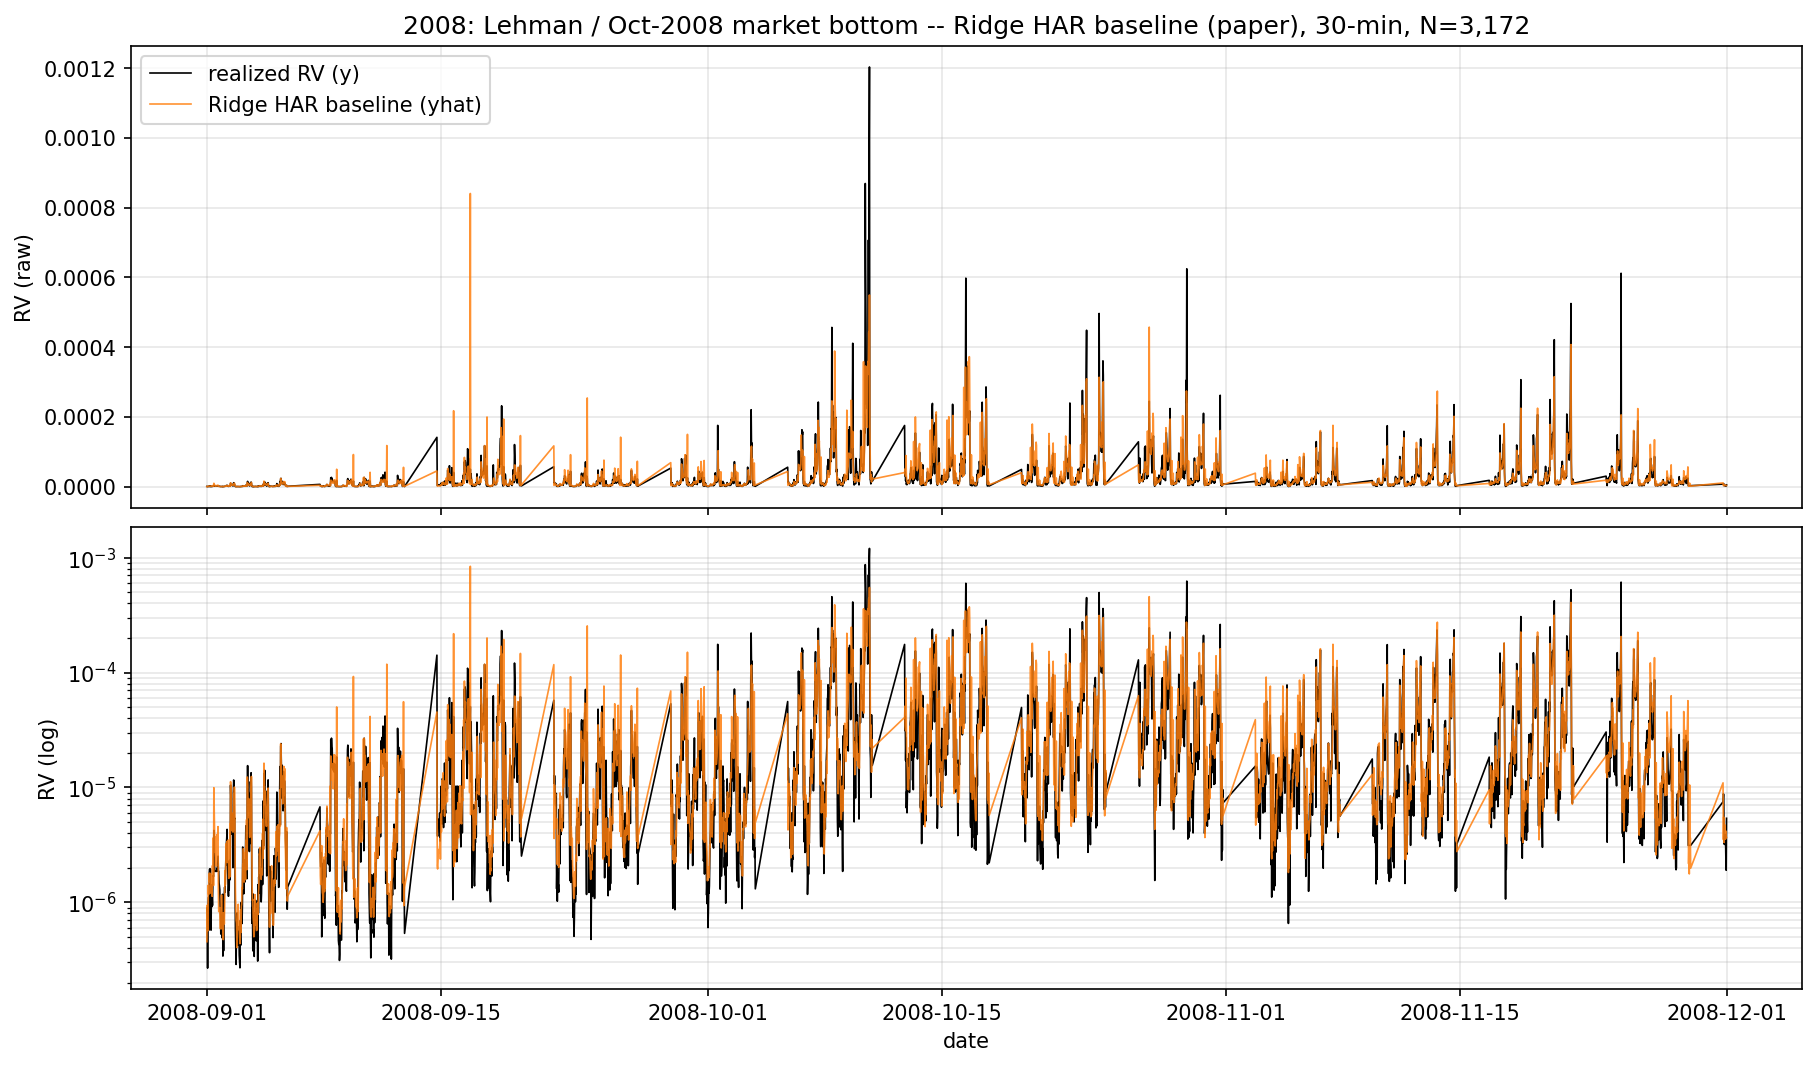
\includegraphics[width=\linewidth]{figures/crash_2008_ridge.png}
\caption{Ridge HAR baseline forecast vs.\ realized $RV$, 30-minute
bars, 2008-09-01 through 2008-11-30. Lehman collapse on 2008-09-15;
TARP; the October 10 equity-market bottom.}
\label{fig:crash_2008}
\end{figure}

\begin{figure}[H]
\centering
% canonical source: results/diagnostics/ridge_har_paper/crash_2020.png
% (writeup/figures/crash_2020_ridge.png is a stale local copy from
%  results/meeting_quickwins/; refresh from diagnostics/ on next build)
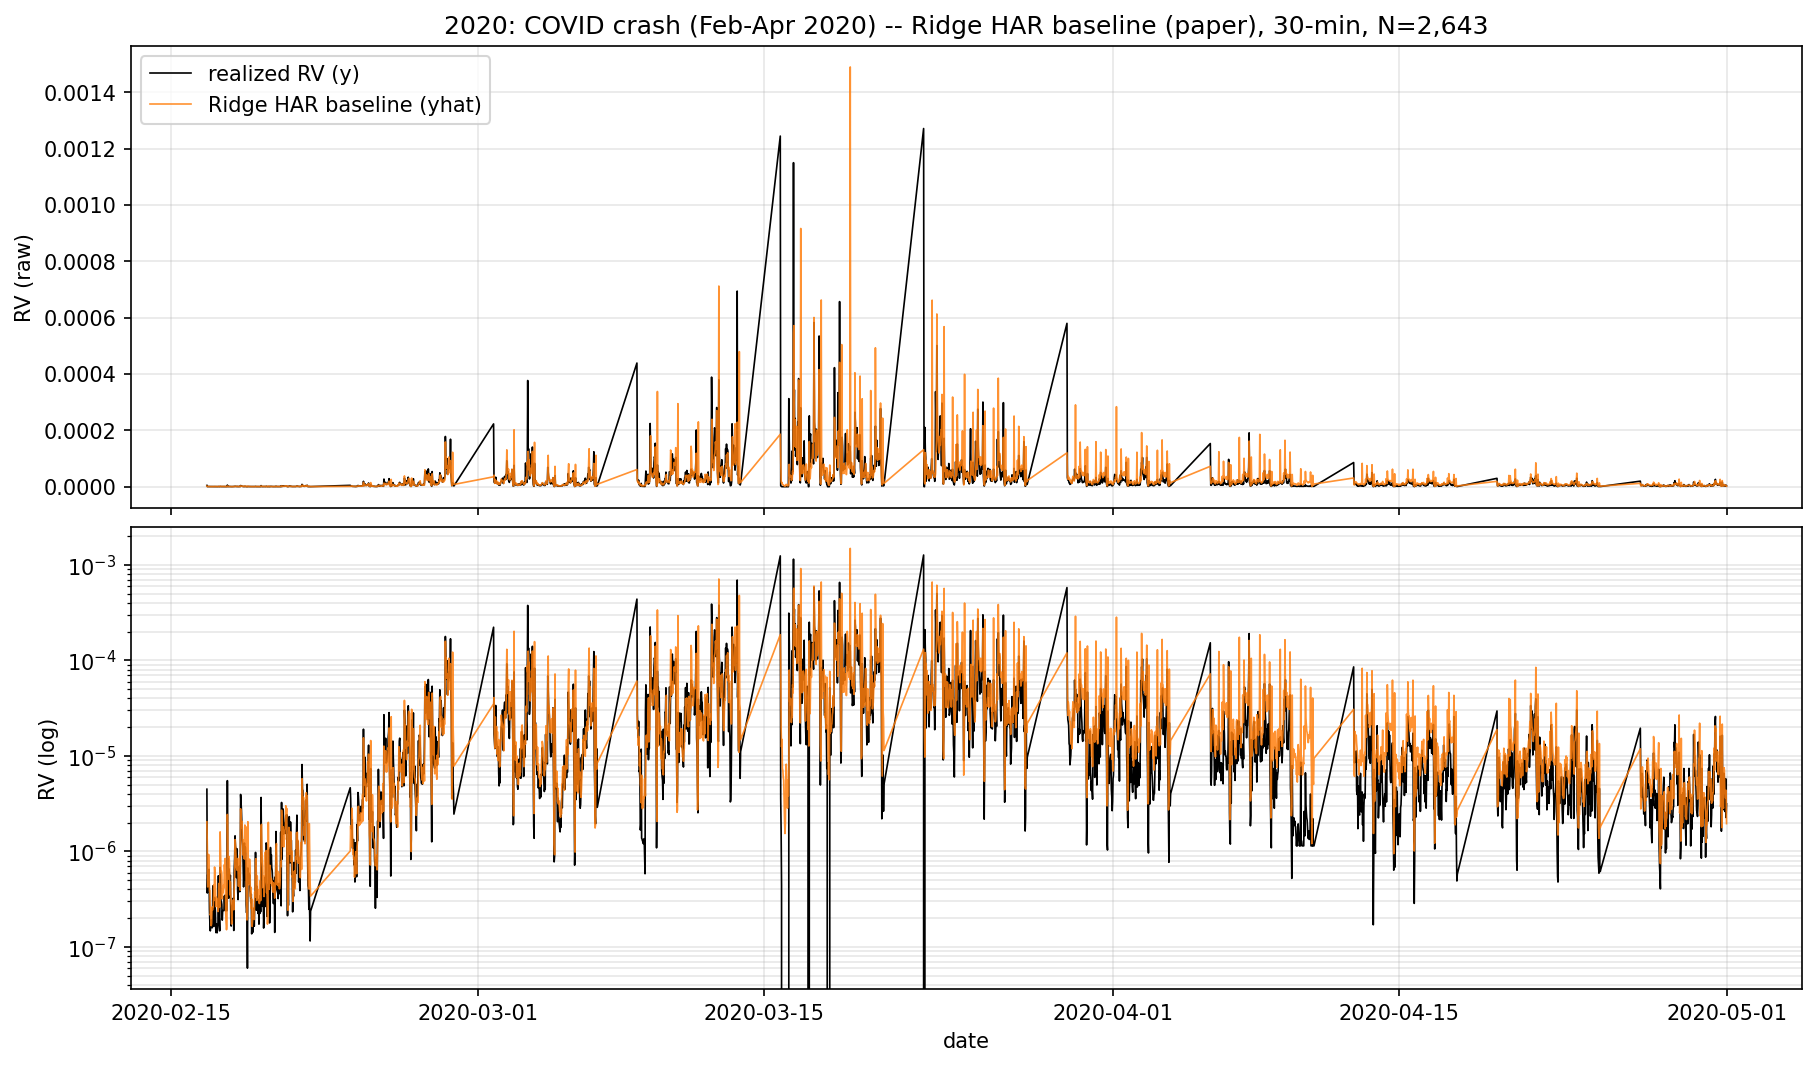
\includegraphics[width=\linewidth]{figures/crash_2020_ridge.png}
\caption{Ridge HAR baseline forecast vs.\ realized $RV$, 30-minute
bars, 2020-02-15 through 2020-04-30. COVID volatility peak around
the March 16 session.}
\label{fig:crash_2020}
\end{figure}

\subsection{Apples-to-apples $N$: the exog ``gain'' revisited}
\label{sec:apples_to_apples}

Prof.\ Jones raised the concern that cross-subgroup QLIKE
comparisons in Table~\ref{tab:ridge_har_subgroup} are contaminated
by differences in $N$ arising from variable-availability-driven
dropna masks. We tested this directly by re-running the ridge HAR
baseline --- target lags only, no exogenous features --- restricted
to the intersection dropna set of the \texttt{liquidity} subgroup.

\begin{table}[H]
\centering
\caption{Apples-to-apples comparison: ridge with and without
liquidity exogenous features, restricted to the same valid-row
subset. Job H2/13131779.}
\label{tab:apples_to_apples}
\begin{tabular}{lrc}
\toprule
Configuration & $N$ & QLIKE \\
\midrule
Ridge + HAR + Liquidity (full dropna) & $203{,}433$ & $0.1317$ \\
Ridge + HAR-only, restricted to liquidity dropna set & $200{,}293$ & $\mathbf{0.1296}$ \\
\bottomrule
\end{tabular}
\end{table}

Once $N$ is matched, the HAR-only configuration is \emph{marginally
better} than the HAR $+$ liquidity configuration. The $6\%$
``liquidity gain'' in Table~\ref{tab:ridge_har_subgroup} is therefore
a dropna-set artifact: the subset of dates for which liquidity
variables are valid is apparently an easier-to-forecast subset, and
attributing that ease to the liquidity features themselves was a
mis-specification. We will replicate this test for every subgroup
in the paper and report intersection-$N$ versions of
Tables~\ref{tab:ridge_har_subgroup}, \ref{tab:model_comparison}, and
\ref{tab:ridge_pca_subgroup} in the next revision.

\subsection{XGBoost vs.\ LightGBM: tuning reliability}
\label{sec:xgb_vs_lgbm_reliability}

At the time of the prior draft, XGBoost had completed $\sim\!4\times$
more Optuna trials than LightGBM (125 vs.\ 30). Diagnostic inspection
of the Optuna storage and per-trial wall times identifies the cause:

\begin{itemize}
    \item LightGBM trials had median wall time $\approx 39$ minutes
      per chunk, versus $\approx 0.7$ minutes for XGBoost --- a
      $55\times$ ratio at the same CPU allocation.
    \item This pushed a substantial fraction of LightGBM trials past
      the SLURM wall-time ceiling, yielding a $59\%$ failure rate
      (versus $34\%$ for XGBoost).
    \item A commit of 2026-04-22 (\texttt{65c85063}) bumped
      per-task CPU allocation and pinned OpenMP thread counts,
      materially improving LightGBM throughput.
\end{itemize}

Even at matched CPU budget, XGBoost remains faster per trial. Two
library-level differences account for this on our problem:

XGBoost's \texttt{tree\_method="hist"} parallelizes histogram construction column-wise, and level-wise tree growth splits $2^{d-1}$ leaves in parallel at each depth. LightGBM's leaf-wise (best-first) growth serializes split decisions, so effective parallelism is lower per tree (leaf-wise vs level-wise parallelism).

We will test whether tightening the LightGBM search space
(\texttt{num\_leaves} $\le 31$, \texttt{max\_depth} $\le 8$,
\texttt{n\_estimators} $\le 500$) combined with
\texttt{early\_stopping\_rounds=50} brings LightGBM failure rates
below $20\%$ and trial times into the XGBoost range.

\subsection{Next steps}
\label{sec:meeting_next_steps}

\begin{enumerate}
    \item \textbf{Intersection-$N$ re-scoring.} Replicate the
      apples-to-apples test for every subgroup and model.
      Rebuild Tables~\ref{tab:ridge_har_subgroup},
      \ref{tab:model_comparison}, \ref{tab:ridge_pca_subgroup} at
      intersection-$N$.
    \item \textbf{Kitchen-sink tree tune.} Launch Optuna on the
      \texttt{all\_features} subgroup for XGBoost and LightGBM; fill
      the missing ``tuned trees $\times$ exog'' cell.
    \item \textbf{SHAP diagnostics} on the winning kitchen-sink XGBoost
      configuration: global feature importance plus dependence /
      interaction plots to localize the source of nonlinear gain at
      the feature level.
    \item \textbf{Volume-regime stratification.} Label each observation
      by a moving-median threshold on \texttt{sumvolume}; report QLIKE
      separately in \texttt{HIGH} and \texttt{LOW} strata as a
      first-pass trading-time-of-day stratification.
    \item \textbf{Regime-change labels.} Condition residuals on
      VIX percentile / realized-vol percentile to make the
      intraday-slot findings robust to regime.
    \item \textbf{Alternative training losses.} Extend the tuning
      driver to support MSE and Huber training objectives
      (retaining QLIKE for evaluation).
    \item \textbf{Option evaluation.} Scope a downstream
      option-pricing backtest (implied-vol error? straddle P\&L?)
      --- advisor input requested on the evaluation target.
\end{enumerate}
